%************************************************Ready v1
\chapter{Frameworks for multi-platform development}\label{ch:frameworks}
%************************************************

%*******DESCRIBE MEANING OF NATIVE***********

There are numerous frameworks that have been developed over the years to facilitate the creation of multi-platform applications. Just like in the 90s, when vendors saw market opportunities in releasing multi-platform applications for the desktop, most of the solutions available for cross-platform mobile development are of the commercial nature.


However, \marginpar{PhoneGap is the commercial name of the Apache Cordova Open Source Project.} some open source players do exist. They have been gaining popularity and better features over time, some have even been backed by bigger organizations, and now offer both free and commercial packages. Examples worth noting in this category are PhoneGap, backed by Adobe\footnote{\url{http://www.adobe.com/}} and Mono, backed by Xamarin\footnote{\url{http://xamarin.com/}}.
\graffito{Mono is an open source implementation of Microsoft's .NET Framework.}

\section{Types of Frameworks}
When it comes to choosing the adequate framework to use for the development of your application, there are many options that vary in number of features, pricing and support; but they can all be sorted into three distinct categories, based on the type of application they produce at the end. These categories are:
\begin{enumerate}
    \item HTML5 Web Applications (\autoref{sec:web_app})
    \item Hybrid Applications (\autoref{sec:hyb_app})
    \item Pseudo-Native Applications (\autoref{sec:pseudo_app})
\end{enumerate}

You should always keep in mind the advantages and drawbacks of each when choosing which type of framework is the best for your needs, but let us take a look at \autoref{tab:frameworks} first. It should give you an overview over the technologies used and the type of applications produced by the most popular cross-platform frameworks. We will discuss each type in detail later on.\newline

\begin{table}[H]
    \myfloatalign
  \begin{tabularx}{\textwidth}{Xll} \toprule
    \tableheadline{Name} & \tableheadline{Language} & \tableheadline{Type}\\ 
    \midrule
    Web frameworks & HTML \& Javascript & Web App\\
    Alloy & HTML, JS \& XML & Hybrid \& Pseudo-Native\\
    Corona SDK & Lua & Pseudo-Native\\
    Embarcadero & Delphi \& C++ & Pseudo-Native\\
    Icenium\textsuperscript{*} & Javascript & Hybrid\\
    Intel XDK\textsuperscript{*} & Javascript & Hybrid\\
    PhoneGap\textsuperscript{*} & Javascript & Hybrid\\
    Rhodes & Ruby \& HTML5 & Hybrid\\
    Titanium & Javascript & Hybrid \& Pseudo-Native\\
    Xamarin & C\# + Native UI & Pseudo-Native\\      
    %\midrule
    \bottomrule
  \end{tabularx}
  \caption[Characteristics of the most popular cross-platform frameworks]{Overview of some characteristics of the most popular cross-platform frameworks\footnotemark}  \label{tab:frameworks}
\end{table}
\marginpar{\vbox{\vspace{-24em}\textsuperscript{*} All of these frameworks are based on Apache Cordova}}
\footnotetext{Information taken from the Framework's respective website}  

As \autoref{tab:frameworks} lets us see, the majority of available frameworks seem to be those that deliver a hybrid application. This phenomenon can be explained by what \citeauthor{allen:2010} express in their book about Cross-Platform Development:
\begin{quotation}
These new smartphone frameworks are influenced by the rapid application development techniques we are seeing in web development today. There are three specific techniques in web application development that are borrowed for these non-web frameworks: 1) layout with mark-up (HTML/CSS); 2) using URLs to identify screen layouts and visual state; and 3) incorporating dynamic languages, such as Javascript and Ruby.

A generation of designers and user interface developers are fluent in HTML and CSS for layout and construction of visual elements. Additionally, addressing each screen by a unique name in a sensible hierarchy (URL) with a systemized way of defining connections between them (links and form posts) has created a lingua franca understood by visual and interactions designers, information architects, and programmers alike. This common language and its standard implementation patterns led to the development of frameworks and libraries that significantly speed application development on the Web. These patterns are now being applied to the development of mobile applications as common techniques by individual developers as well as in cross-platform frameworks.
\cite[p. 23]{allen:2010}
\end{quotation}
Before we dive into each type of framework, \autoref{fig:hybrid_native} should give you a better overview over their capabilities.\\

\marginpar{The 'Native' label also applies to Pseudo-Native}
\begin{figure}[H]
    \begin{center}
        {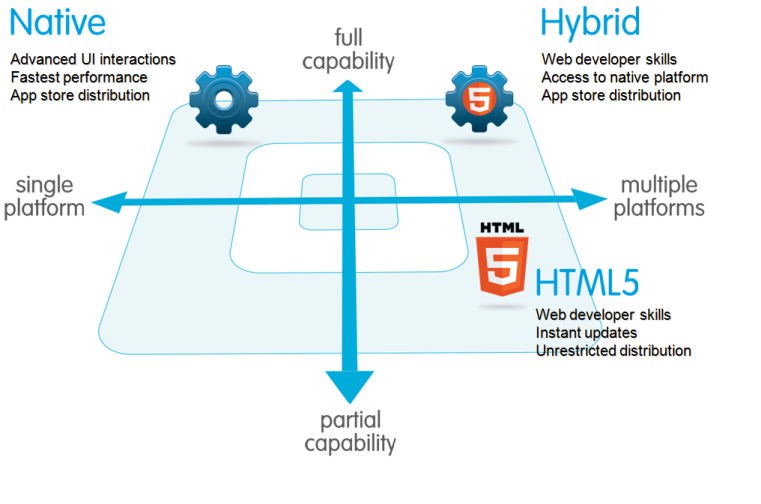
\includegraphics[width=1\linewidth]{gfx/Native_html5_hybrid}}
        \caption[Overview of app capabilities. Native vs. Hybrid vs. HTML5]{Overview of app capabilities. Native vs. Hybrid vs. HTML5\footnotemark}\label{fig:hybrid_native}
    \end{center}
\end{figure}
\footnotetext{Source: \url{http://wiki.developerforce.com/page/Native,_HTML5,_or_Hybrid:_Understanding_Your_Mobile_Application_Development_Options}}\\

\subsection{HTML5 Web Applications}\label{sec:web_app}
Just as any other website, \spacedlowsmallcaps{HTML5 Web Applications} can be developed in any language that can be translated to HTML code on runtime. Some examples of these languages are \emph{Ruby, PHP, Python, JSP} or just plain HTML. Some of the most popular web development frameworks, like Ruby on Rails or Synfony\marginpar{Synfony is an MVC Framework for PHP, similar, but not quite as powerful as Rails.}, are very well suited for the development of Web Applications for Mobile Devices.


But having HTML code is not everything, you still need to make it look good in the smaller screen of cellphones and tablets. That's where CSS3\footnote{\url{http://www.w3schools.com/css/css3_intro.asp}} comes into play. With CSS3 you define the look and feel of the application, but you need to define specific rules for devices with a smaller resolution. This can be accomplished in two ways:
\begin{enumerate}
    \item Responsive CSS3 Design
    \item Separate Domain and CSS files for mobile devices
\end{enumerate}
\spacedlowsmallcaps{Responsive CSS3 Design} means you need to distinguish between the different screen sizes and define different rules and properties for each inside your CSS files. With responsive design, changes in screen orientation can also be translated to a different layout, e.g. changing the width of tables or the arrangement of images.


With \spacedlowsmallcaps{Separate Files} you will have to redirect visitors using a mobile device to a different domain and have that domain serve the corresponding CSS files. This approach has some caveats, the most obvious one being the overhead of a different domain with separate HTML and CSS files to maintain and the fact that if you want your layout to react to screen dimension changes, you will most likely need to implement some sort of responsive design, anyway.   
 

These frameworks, however, cannot run inside the mobile device; they need to run on a server, which means that the only way to access the application is through a web browser.


This line of action is best suited for smaller projects that want to present their website or web application in a better way to mobile users, but don't have the resources to hire a full time application developer. They can use the designer they have at hand and just optimize their online presence for portable devices.

\subsection{Hybrid Applications}\label{sec:hyb_app}
\begin{quotation}
Before any cross-platform frameworks existed, many developers found that embedding a Web \ac{UI} in a native application was a practical way to develop mobile applications quickly and make cross-platform applications easier to maintain. The user interface for mobile applications tends to be presented as a series of screens. From a high level, the mobile \ac{UI} can be thought of as having the same flow-of-control as a traditional web site or web application. \cite[p. 28]{allen:2010}
\end{quotation}

\spacedlowsmallcaps{Hybrid Applications} are, in a lot aspects, very similar to HTML5 Web Applications. Both rely on HTML, Javascript and CSS for the definition of the \ac{UI}, but the edge of Hybrid Applications lies in the way they are packaged.

With Hybrid Applications the HTML, et al. are contained within a native package, that allows the framework's \ac{API} to communicate with the operating system, thus leveraging some of the native features the hardware has to offer, e.g. access to the camera, the accelerometer, the GPS, local storage, etc. Access to these features is accomplished via a wrapper that is programmed in each platform's native language and exposes specific methods to an \ac{API} that is accessible from the HTML side using Javascript methods.

By having access to these features, Hybrid Applications can behave like native applications and, since they are contained within a native package, there is no need for the user to open a web browser. It also gives you the advantage of distributing your application via the platform's store.

This approach gives you many added benefits over a normal HTML5 Application, with just some trade-offs. There is a learning curve involved when dealing with the programming frameworks, but the design and layout are still done in HTML and CSS. One of the main benefits you get is that you now have the possibility to make your application available offline and of course the access to system features, like push notifications. 

The downside is that every piece of the \ac{UI} \textsc{needs} to be done in CSS and HTML. There are no native controls, so your application will not look exactly as a native application, and some very important native features may not be available to you. Depending on the framework you choose, you may not have access to security features, like encryption of resources, or low level features, like background services.  

This approach is best suited for projects that want to offer more functionality with their mobile applications and are willing to invest some time in learning a new framework.  

\subsection{Pseudo-Native Applications}\label{sec:pseudo_app}
\spacedlowsmallcaps{Pseudo-Native Applications} are completely different from the other two types. They do not rely on HTML for the \ac{UI}. These applications are \textsc{compiled} to native code (in most frameworks) and appear to the device as native.


The way the \ac{UI} is programmed varies between the different frameworks. It can be done using the native tools of each platform; using a visual designer provided by the framework or programmatically, using the libraries provided.

Independently from which method is used for the \ac{UI}, the business logic is always done separately in an effort to abstract as much shared functionality as possible and keep platform specific code to a minimum.

One of the downsides of taking this approach, is that you have to program the \ac{UI} separately for each platform, which translates into more work and somewhat less maintainability. The advantages, however, can offset all the extra effort.

Let's take a look at the advantages offered by this type of applications:

\begin{description}

\item[Speed:] Depending on the framework you choose, your entire code can be compiled to native binaries, thus performance can be increased. This is crucial for applications that need to do a lot of calculations quickly or that rely on the assessment of large amounts of data.

\item[Flexibility:] Since the \ac{UI} code is not shared between platforms, it gives you the flexibility to adapt and modify the layout of your application depending on which device is running it. It also gives your application a truly native look \& feel and not an emulated one.

\item[Extra Features:] There are some device features that are not available via Wrapper \ac{API}s but can be accessed by these frameworks, either by extra libraries or by manually extending the framework with native code. This gives you complete control over what you application is capable of doing.
 
\item[Code Reusability:] If you have external libraries that you would like to include in your project, but don't want to rewrite them, using one of these frameworks allows you to include them in your application if they are programmed in C or C++. 

\end{description}

Using this approach is by no means easy and requires a lot of time and resources, which most often translates into money. But if you want to have complete control over your project, have code that you want to reuse or you simply need your application to run at full speed, this is the right line of action for you.